% VUT FIT MITAI
% MSZ 2021/2022
% Author: Vladimir Dusek
% Login: xdusek27

%%%%%%%%%%%%%%%%%%%%%%%%%%%%%%%%%%%%%%%%%%%%%%%%%%%%%%%%%%%%%%%%%%%%%%%%%%%%%%%%

% Path to figures
\graphicspath{{sui/neuronove_site_pro_strukturovana_data/figures}}

%%%%%%%%%%%%%%%%%%%%%%%%%%%%%%%%%%%%%%%%%%%%%%%%%%%%%%%%%%%%%%%%%%%%%%%%%%%%%%%%

\chapter{SUI~--~Neuronové sítě pro strukturovaná data (konvoluční a rekurentní sítě, motivace, základní vlastnosti, použití).}

%%%%%%%%%%%%%%%%%%%%%%%%%%%%%%%%%%%%%%%%%%%%%%%%%%%%%%%%%%%%%%%%%%%%%%%%%%%%%%%%

\section{Zdroje}

\begin{compactitem}
    \item \path{09-neural_networks.pdf}
    \item \path{10-sequences_and_language.pdf}
    \item \path{SUI_2019-12-02.mp4}
    \item \path{SUI_2019-12-09.mp4}
\end{compactitem}

%%%%%%%%%%%%%%%%%%%%%%%%%%%%%%%%%%%%%%%%%%%%%%%%%%%%%%%%%%%%%%%%%%%%%%%%%%%%%%%%

\section{Strukturovaná data}

\begin{compactitem}
    \item Za strukturuovaná data považujeme obrázky, zvuk, text, \dots \begin{compactitem}
        \item Mají nějakou strukturu, nejsou to neuspořádaná data.
    \end{compactitem}

    \item Standardní vícevrstvé neuronové sítě by fungovali i pro tyto data, avšak lze využít vlastností strukturovaných dat, pro efektivnější práci neuronových sítí.

    O jaké vlastnosti jde: \begin{compactitem}
        \item \textbf{Lokalita} -- V případě obrázku, pixely, které se vyskytují blízko sebe, pravděpodobně patří stejnému objektu. Naopak pixely daleko od sebe spíše nepatří.

        \item \textbf{Invariance zpracování vzhledem k pozici} -- V případě obrázku, vychází myšlenky, že objekty v obraze se mohou pohybovat. Pokud se určitý objekt detekuje na jednom místě, je možné ho stejným způsobem detekovat i na jiném místě.
    \end{compactitem}

    \item Další specifické vlastnosti mají sekvence (video, zvuk) -- časovou souvislost.
\end{compactitem}

%%%%%%%%%%%%%%%%%%%%%%%%%%%%%%%%%%%%%%%%%%%%%%%%%%%%%%%%%%%%%%%%%%%%%%%%%%%%%%%%

\section{Konvoluční neuronové sítě}

\begin{compactitem}
    \item Konvoluční neuronové sítě (CNN, \textit{convolutional neural networks}) jsou hluboké neuronové sítě, ve kterých jednotlivé skryté vrstvy mají formu zaměření pro konkrétní činnost (konvoluce, pooling,dropout, \dots).
\end{compactitem}

\subsection{Konvoluční vrstvy}

\begin{compactitem}
    \item Konvoluční vrstvy (\textit{convolutional layers}) jsou hlavní stavební kameny konvolučních neuronových sítí. Jejich název je převzat od jména matematické operace, která se ve vrstvě provádí -- konvoluce ($\star$). \begin{compactitem}
        \item Jde o operaci, která dokáže dobře využít vlastnosti strukturovaných dat (lokalita, invariance zpracování vzhledem k pozici).

        \item Obraz je reprezentován diskrétními hodnotami pixelů, konkrétně maticí těchto hodnot, proto nás zajímá diskrétní 2D~konvoluce.

        \begin{equation}
            f(x,y) \star h(x,y)=\sum_{i=-k}^{k}\sum_{j=-k}^{k}f(x-i,y-j)\cdot h(i,j)
        \end{equation}

        \item Symbol $\star$ je operátor konvoluce nad funkcemi $f(x,y)$ a $h(x,y)$. První operand, v~našem případě funkce $f$, obvykle značí vstupní obraz a druhý operand, funkce $h$, značí konvoluční jádro (filtr).
    \end{compactitem}

    \item Intuice, která stojí za aplikací konvoluce, je hledání podobnosti tzv. konvolučního jádra (konvoluční filtr) a daného segmentu obrazu. Výsledkem je, jak velký má být signál daného segmentu v rámci celého výsledku.

    % \item Konvoluční vrstva se typicky skládá z několika různých konvolučních jader.

    \item Obrázek je typicky reprezentován maticí hodnot pixelů pro každý barevný kanál (pokud není v odstínu šedi). Konvoluce se aplikuje na každý barevný kanál.

    \item Parametry konvoluční vrstvy se skládají z~množiny \textbf{konvolučních filtrů}. Samotná síť se učí optimalizací jejich jednotlivých hodnot. Filtry jsou po vstupu posouvány po určitém kroku a je počítána výsledná dvoudimenzionální mapa. Konvoluční filtry mohou mít různá uplatnění. Například pro rozmazaní či doostření obrazu, ale také pro  detekci hran. Hrana je rozpoznána prudkou změnou světelných podmínek. Podstata filtru je nalézt gradient, tj. směr maximální změny, který hranu charakterizuje.

    \item Výstupní matice je menší než vstupní. To je důsledkem toho, že pro výpočet jednoho výsledného bodu potřebujeme na vstupu matici o~velikosti filtru. Pokud chceme zmenšení rozlišení předejít, dá se původní matice rozšířit. A~to buď nulovými body (\textit{zero padding}), případně jinými, vhodně vybranými hodnotami. Avšak většinou je zmenšení žádané, výstup je jiný obrázek, resp. jeho jiná (jednodušší) reprezentace.

    \item Vlivem výpočtu v~konvolučních vrstvách může dojít k~tomu, že některé hodnoty v~matici nabudou záporných hodnot. Barvy jsou ale reprezentovány třemi kanály v~rozmezí~0\,--\,255. Proto je často používána přenosová funkce ReLU, která odstraní negativní hodnoty z~aktivační mapy.
\end{compactitem}

\begin{figure}[H]
    \centering
    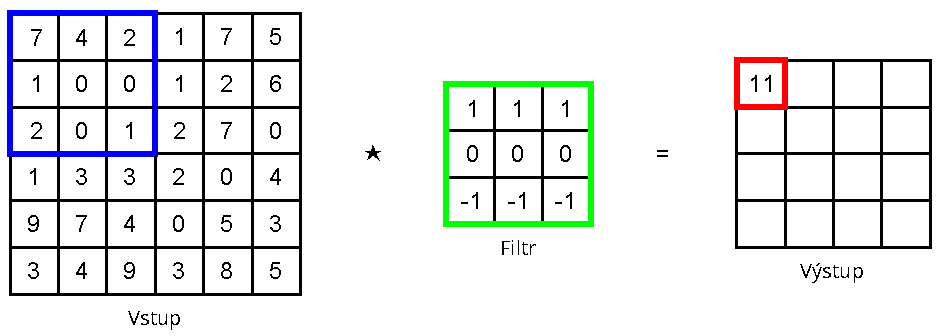
\includegraphics[width=0.8\linewidth]{convolution.pdf}
    \caption{Příklad aplikace konvoluce.}
\end{figure}

\begin{figure}[H]
    \centering
    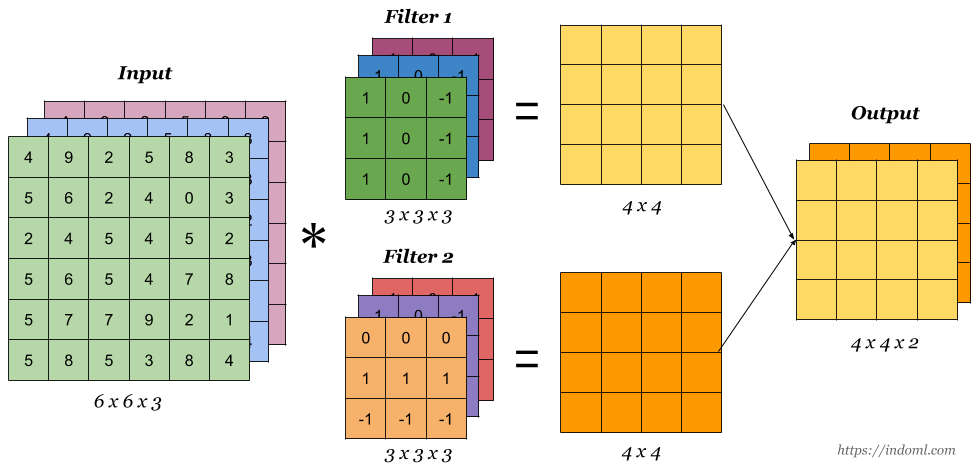
\includegraphics[width=1\linewidth]{conv.png}
    \caption{Příklad aplikace konvoluce, vstup má 3 barevné kanaly, vrstva obsahuje 3 konvoluční filtry.}
\end{figure}

\begin{figure}[H]
    \centering
    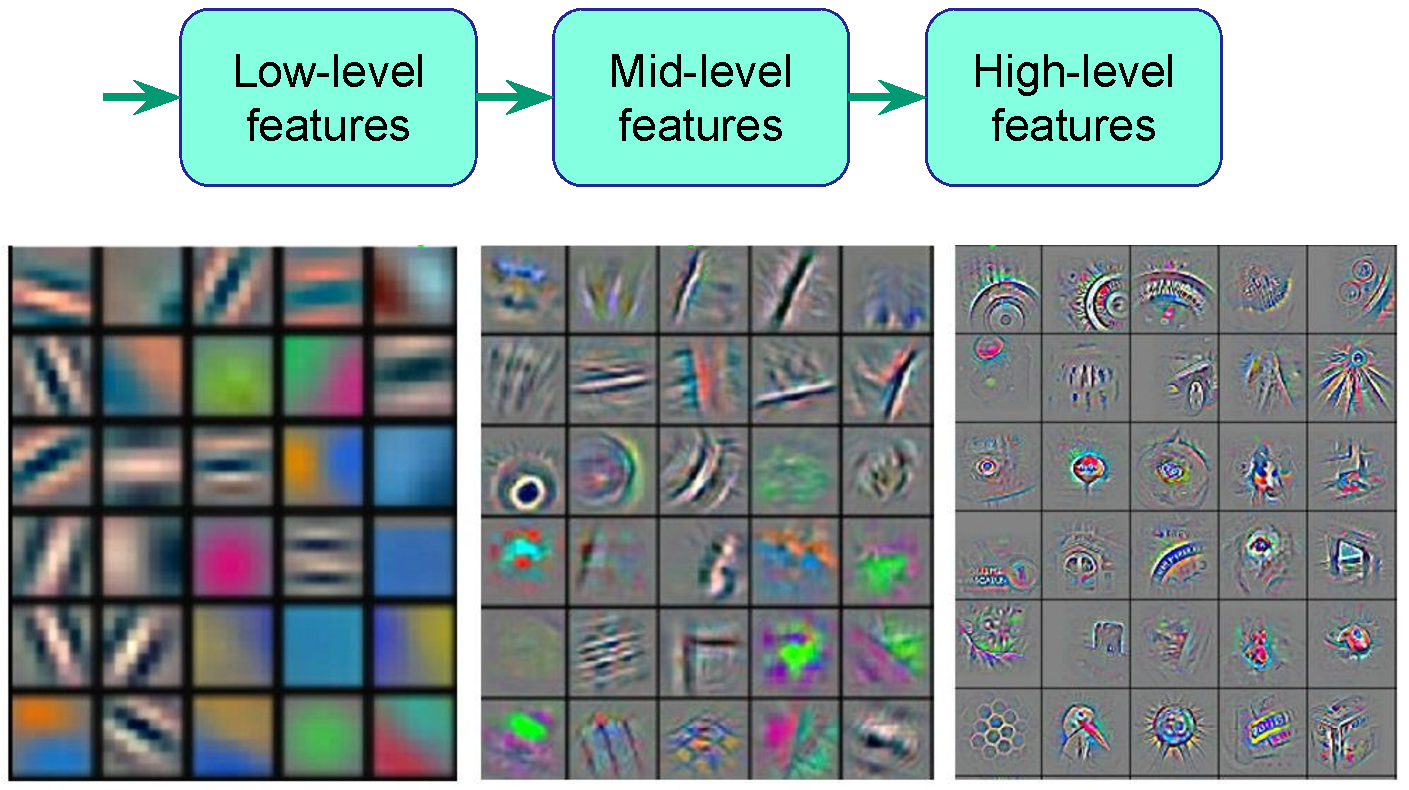
\includegraphics[width=0.75\linewidth]{conv-kernel.pdf}
    \caption{Příklad konvolučních jader.}
\end{figure}

\subsection{Pooling vrstvy}

\begin{compactitem}
    \item Sdružování (\textit{pooling}), slouží pro podvzorkování~--~zmenšení rozměrů dvoudimenzionální mapy.

    \item Díky tomu, se zmenší počet parametrů sítě v dalších vrstvách a dojde ke snížení výpočetních nároků.

    \item Realizuje se agregací několika sousedních buněk do jedné. Nejběžnější způsoby jsou \textit{average pooling}, kdy se počítá průměrná hodnota z~agregovaných buněk a \textit{max pooling}, kdy se vybírá maximální hodnota.

    \item Pooling vrstvy nemají parametry (neučí se), jsou natvrdo naprogramované.

    \item Za sdružováním stojí myšlenka, že úplně přesná lokace příznaku není pro úlohu důležitá. Naopak může být na škodu a podpořit problém přetrénování sítě. Důležitější je tedy relativní lokace příznaku vzhledem k~ostatním. Tím se dosáhne větší obecnosti modelu (generalizace).

    \item Pooling vrstva se běžně vkládá mezi jednotlivé konvoluční vrstvy. V~současnosti se nejvíce používá přístup \textit{max pooling} a \textit{average pooling}.
\end{compactitem}

\begin{figure}[H]
    \centering
    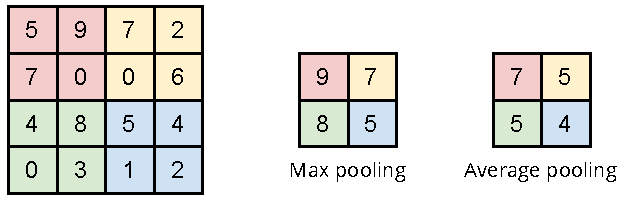
\includegraphics[width=0.7\linewidth]{pooling.pdf}
    \caption{Příklad aplikace max a average poolingu.}
\end{figure}

\subsection{Plně propojená vrstva}

\begin{compactitem}
    \item Plně propojená vrstva (\textit{fully connected layer} nebo \textit{dense layer}) spojuje každý neuron z~dané vrstvy s~každým neuronem vrstvy následující.

    \item Jedná se o~stejný princip jako u~klasických vícevrstvých neuronových sítí.

    \item Ačkoliv jsou sítě s~plně propojenými vrstvami schopny dobře aproximovat libovolnou funkci, jejich vysoký počet spojení výrazně zvyšuje nároky na výpočetní kapacity. Proto se vyskytují spíše až v~koncových vrstvách konvolučních sítí, kde mají na starosti klasifikaci objektů.
\end{compactitem}

\subsection{Dropout vrstva}

\begin{compactitem}
    \item Dropout vrstva má za úkol snížit náchylnost sítě k~přetrénování.

    \item Spočívá v~nastavení výstupu každého neuronu ve skryté vrstvě na~0 s~pravděpodobností~50\,\% (tzv. deaktivace neuronu).

    \item K~deaktivaci neuronů dochází u~každého vzorku dat při trénování, do učení je tak uměle přidáván šum, díky kterému je síť schopna více generalizovat.

    \item Dropout vrstva zvýšuje počet potřebných iterací k~dosažení konvergence.
\end{compactitem}

\subsection{Loss vrstva}

\begin{compactitem}
    \item Za poslední typ vrstvy lze považovat \textit{loss} vrstvu, která specifikuje jak proces trénování penalizuje rozdíl mezi predikcí sítě (výstupem) a skutečnými hodnotami (označená trénovací data) -- chybové funkce (objektivní funkce).

    \item Jedná se o~finální vrstvu neuronové sítě.

    \item Existuje mnoho chybových funkcí určené pro různé typy úloh.
\end{compactitem}

\subsection{Příklady architektur}

\begin{figure}[H]
    \centering
    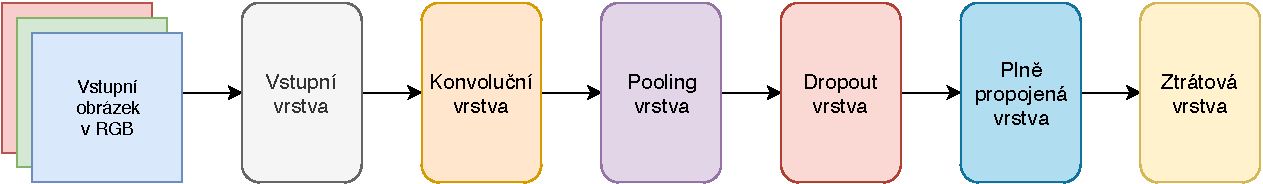
\includegraphics[width=1\linewidth]{conv-arch.pdf}
    \caption{Příklad uspořádání jednotlivých typů vrstev za sebe. Typicky konvoluční a pooling (potažmo dropout) vrstvy se několikrát opakují.}
\end{figure}

\begin{figure}[H]
    \centering
    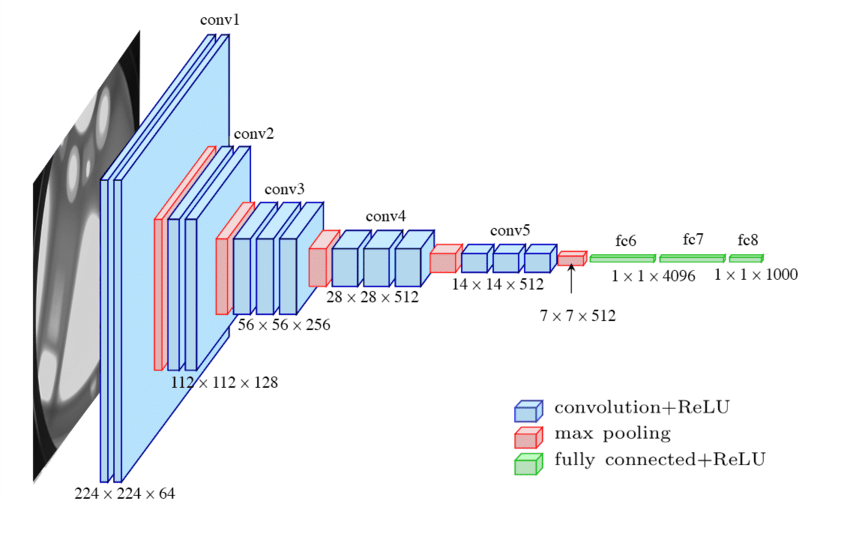
\includegraphics[width=1\linewidth]{vgg.png}
    \caption{Příklad konvoluční neuronové sítě VGG pro klasifikaci obrazu (vstupní a ztrátová vrstva nejsou ve schématu zobrazeny). Čím hlubší vrstva, tím menší matice, ale o to více konvolučních filtrů.}
\end{figure}

%%%%%%%%%%%%%%%%%%%%%%%%%%%%%%%%%%%%%%%%%%%%%%%%%%%%%%%%%%%%%%%%%%%%%%%%%%%%%%%%

\section{Rekurentní neuronové sítě}

\begin{compactitem}
    \item Základní vícevrstvé NN i konvoluční NN patří mezi tzv. dopředné neuronové sítě.

    \item Rekurentní NN jsou další kategorií, která narozdíl od dopředných NN nepropaguje signál výhradně do dalších vrstev. \begin{compactitem}
        \item Resp. rekurentní vrstvy nejsou acyklické, ale obsahují jakýsi \textit{self loop}.
    \end{compactitem}

    % \item Specifikem strukturovaných dat v rámci videa nebo zvuku je kombinace prostorové i časové souvislosti, v tom nám vnitřní stav neuronu pomůže.

    \item U výpočtu odezvy perceptronu je využito kromě aktuálního vstupu i vnitřní stav perceptronu. \begin{compactitem}
        \item
        Resp. jsou využity informace z předchozích vstupů, které jsou zakódovány ve vnitřním stavu.
    \end{compactitem}

    \item Rekurentní NN dokáží zachytit vlastnosti časové souvislosti v rámci sekvence dat.

    \item Rekurentní NN mají problém se naučit dlouhodobé závislosti.
\end{compactitem}

\begin{figure}[H]
    \centering
    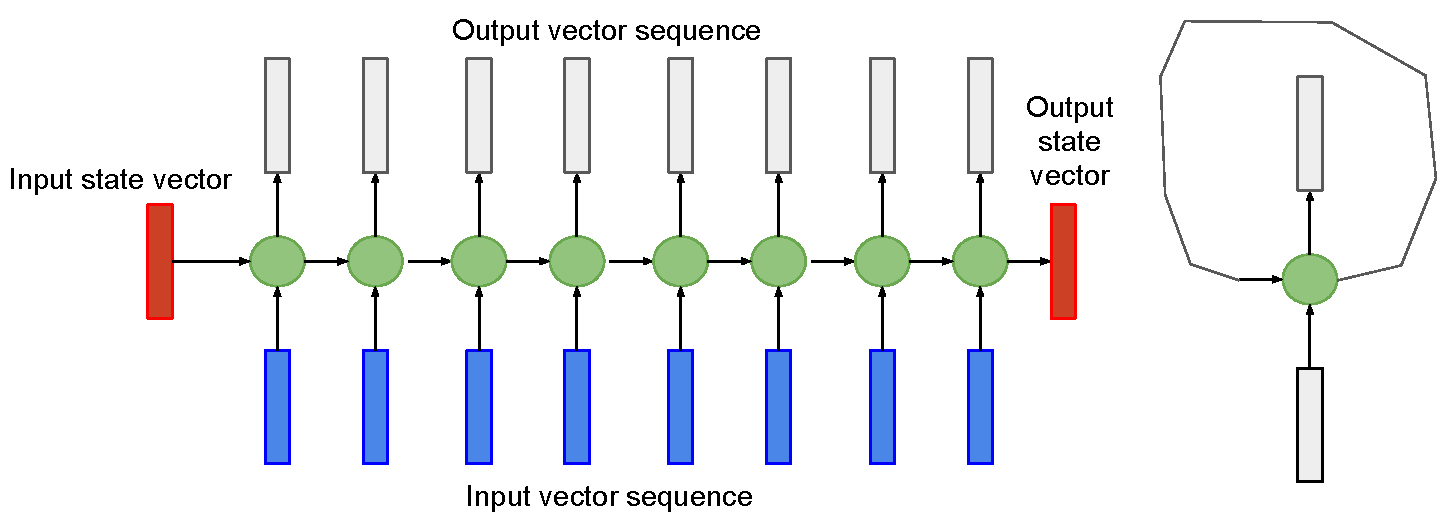
\includegraphics[width=1\linewidth]{recurrent.pdf}
    \caption{Vizualizace rekurentní vrstvy. Výstup vrstvy jde na vstup stejné vrstvě v další iteraci.}
\end{figure}

\subsection{Vanilla RNN}

\begin{compactitem}
    \item První model rekurentní NN, základní model.
\end{compactitem}

\begin{figure}[H]
    \centering
    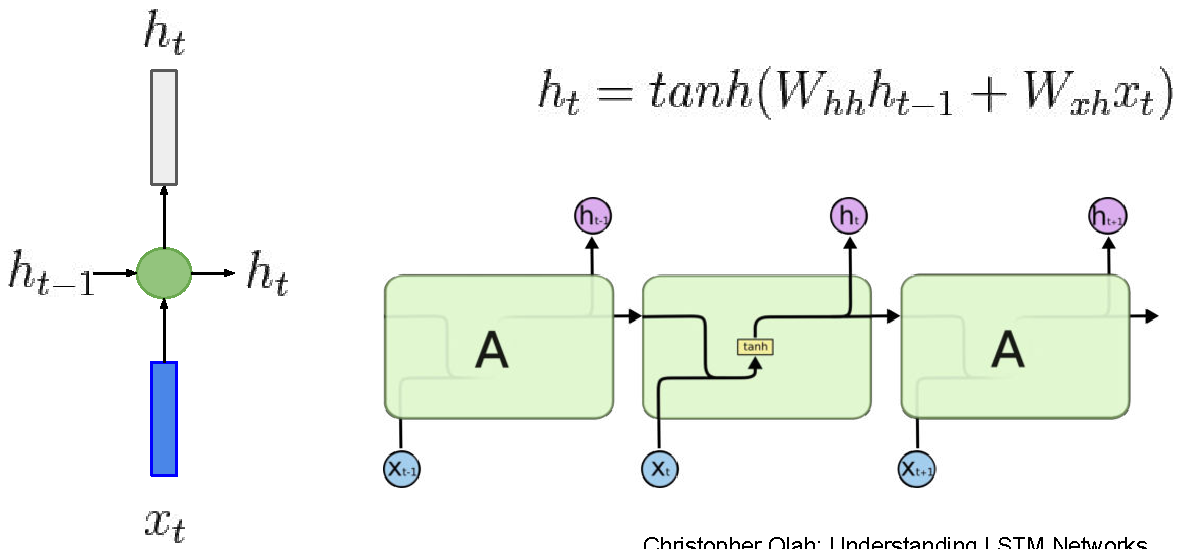
\includegraphics[width=1\linewidth]{rnn-vanilla.pdf}
    \caption{Schéma Vanilla RNN.}
\end{figure}
